\chapter{Extendiendo el borrow checker}

\section{Entendiendo los procesos del compilador}

El compilador de Rust según \cite{rustcdevelopment} se diferencia del resto, ya que hace procesos que otros no realizan (borrow-checking) y también toma algunas decisiones no convencionales. El proceso de compilación de un programa comienza al invocar el comando \textbf{rustc} junto al código fuente de un programa y los parámetros. El modulo \textit{rustc\_driver} se encarga de captar los argumentos y definir la configuración que se utilizará en el resto del procedimiento.

Una vez que el compilador captó el código, los módulos \textit{rustc\_lexer} y \textit{rustc\_parse} se encargan de analizarlo y generar el AST (árbol de sintaxis abstracta). En esta primera etapa también se expanden las macros, se resuelven los nombres, se chequea la sintaxis del programa y se valida que el AST sea correcto.

\begin{wrapfigure}{r}{0.25\textwidth}
    \caption{Compiler pipeline}
    \centering
    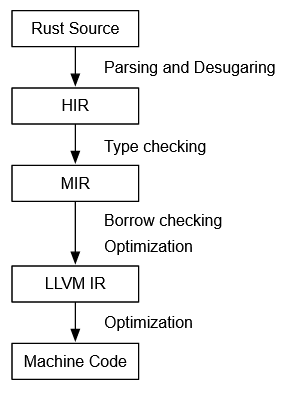
\includegraphics[width=0.3\textwidth]{compiler-flow}
\end{wrapfigure}

Teniendo este árbol, se proceden a generar las representaciones intermedias. La primera en construirse es el HIR ( High-Level Intermediate Representation) que es una version más amigable para el compilador del AST. Durante este proceso se realiza la inferencia de tipos, la resolución de las traits y principalmente el chequeo de tipos, donde se convierten los tipos encontrados en el HIR por representaciones internas usadas por el compilador. Estas son usadas para aumentar la seguridad, correctitud y coherencia de los tipos utilizados en el programa.

La siguiente parte es la construcción del MIR (Mid-Level Intermediate Representation) a partir del HIR. Aquí es donde se hacen gran parte de las optimizaciones del código, junto al pattern-matching y chequeos de exhaustividad. Además, el MIR es donde se realiza el \text{borrow-checking} y otros chequeos importantes basados en el flujo de datos. Debido a que es una representación de alto nivel y genérica es aquí donde se realizan la mayoría de análisis del compilador, y nosotros tomaremos en cuenta esto para añadir nuestros propios algoritmos y análisis.

A continuación se realiza lo que es conocido por la generación de código o \textit{codegen}, que consiste en transformar las representaciones de alto nivel a un binario executable. \textbf{rustc} utiliza \textbf{LLVM} para esto. Se comienza convirtiendo el MIR en LLVM IR (LLVM Intermediate Representation) para luego pasárselo a LLVM, el cual realiza más optimizaciones, y emitir el código de maquina. Este es básicamente código assembler con algunos tipos y anotaciones añadidos. Los diferentes binarios/bibliotecas luego son unidos (linked) para crear el binario final.

\section{Análisis estáticos sobre el MIR}

\subsection{MIR}

\cite{rustcdevelopment} dice el MIR que es una forma simplificada de Rust el compilador utiliza principalmente para comprobaciones de seguridad flow-sensitive, como por ejemplo el borrow checker. Esta definido en el modulo \textbf{rust\_middle::mir}, se basa en un CFG (Control-Flow Graph o Grafo de Control de Flujo) y todos los tipos son explícitos.

El CFG es un término común en el ámbito de los compiladores, ya que permite representar un programa exponiendo de manera clara el flujo del mismo. El CFG del MIR esta estructurado como un conjunto de bloques básicos conectados por aristas. Estos bloques básicos están conformados por un conjunto de \textit{statements} que se ejecutarían juntos y de manera secuencial y completa. Al final se encuentra un \textit{terminator} cuya función es referenciar y conectar bloques básicos. La construcción de un CFG es generalmente el primer paso de la mayoría de los algoritmos de análisis flow-sensitive, y el MIR esta estructurado de esta manera para facilitar estos análisis.

Otros conceptos claves del MIR son:
\begin{itemize}
    \item \textbf{Locals}: Lugar de la memoria alojado (conceptualmente) en el stack. Se representan con un guion bajo seguido de un numero, por ejemplo \_1. El lugar \_0 esta reservado para la dirección de retorno de la función.
    \item \textbf{Places}: Expresiones que identifican un lugar en la memoria.
    \item \textbf{Rvalues}: Expresiones que producen un valor. Su nombre proviene del hecho de que están del lado derecho de una asignación.
    \begin{itemize}
        \item \textbf{Operands}: Son los argumentos de un rvalue, que pueden ser constantes o Places
    \end{itemize}
\end{itemize}

Mediante el uso de las versiones nightly del compilador, que añaden la posibilidad de importar módulos críticos e imperativos para los análisis estáticos que queremos realizar, es posible acceder y utilizar las distintas representaciones intermedias de un código fuente.

Podemos apreciar la transformación a MIR mediante un ejemplo. El siguiente programa básico
\begin{lstlisting}[language=Rust]
    fn main() {
        let mut x = 5;
        x = x + 10;
    }
\end{lstlisting}
tiene una representación en MIR de la siguiente forma:
\begin{lstlisting}[language=Rust]
    // WARNING: This output format is intended for human consumers only
    // and is subject to change without notice. Knock yourself out.
    fn main() -> () {
        let mut _0: ();            // return place in scope 0 at ./examples/simple_sum.rs:1:11: 1:11
        let mut _1: i32;           // in scope 0 at ./examples/simple_sum.rs:2:9: 2:14
        scope 1 {
            debug x => _1;                   // in scope 1 at ./examples/simple_sum.rs:2:9: 2:14
        }

        bb0: {
            _1 = const 5_i32;      // scope 0 at ./examples/simple_sum.rs:2:17: 2:18
            _1 = const 15_i32;     // scope 1 at ./examples/simple_sum.rs:3:5: 3:15
            return;                // scope 0 at ./examples/simple_sum.rs:4:2: 4:2
        }
    }
\end{lstlisting}

Este ejemplo, como indica el comentario arriba, muestra el MIR para que sea más sencillo de leer por las personas. Podemos apreciar como se crea la función main, se realizan las declaraciones de las variables en la parte superior y luego procede a definirse los bloques básicos. En este caso, el bloque bb0 es el único que se construyo y contiene dos statements y un terminator. Debido a la optimizaciones del compilador (expansión de constantes), los statements son solo asignaciones directas sin la necesidad de hacer una suma como en el programa fuente. El terminator en este caso es la llamada a return.

Para extender el borrow checker, se realiza una interpretación abstracta del MIR aplicando los análisis estáticos necesarios y recopilando la información.
